\documentclass[pdf]{ifacconf}


\usepackage{amsmath}
\usepackage{natbib}            % you should have natbib.sty
\usepackage{graphicx}          % Include this line if your 
                               % document contains figures,
%\usepackage[dvips]{epsfig}    % or this line, depending on which
                               % you prefer.
                               
\usepackage{units}
%\usepackage{babelbib}
%\bibliographystyle{babunsrt}

% for German
\usepackage{ngerman}           % neue Deutsche Rechtschreibung, Silbentrennung
\usepackage[UTF8]{inputenc}  % Eingabe von Umlaute im Editor
%\usepackage[T1]{fontenc}       % Trennung mit Umlauten

\usepackage{tikz,pgfplots}
\pgfplotsset{compat=newest} 
\usetikzlibrary{shapes,arrows,positioning,arrows.meta}


\begin{document}

\begin{frontmatter}

\title{``Projektwettbewerb Einführung in die Regelungstechnik'' - Stabilisierung eines Segways auf einer Wippe}

%\thanks[footnoteinfo]{Institute for Systems Theory and Automatic Control, University of Stuttgart, Germany. \textit{http://www.ist.uni-stuttgart.de}}

% include all authors, underline corresponding author
%\author{\underline{},} 
%\author{Alessio Gaggiano (Kyb 3129632), Shadi Rafe (Kyb ********), Truc-Quynh Doan (Kyb 3152793)}  %passt nicht rein 
\textbf{\makebox[\linewidth][c]{Alessio Gaggiano (Kyb 3129632), Shadi Rafe (Kyb 2922872), Truc-Quynh Doan (Kyb 3152793)}}

\begin{abstract}\\                          % Abstract of not more than 250 words.
Die folgende Dokumentation beinhaltet die ausführliche Beschreibung unseres Lösungsansatzes und der Ergebnisse der regelungstechnischen Aufgabe ``Stabilisierung eines Segways auf einer Wippe''. 
%This is a template for the laboratory course ``Projektwettbewerb Einführung in die Regelungstechnik'' at the Institute for Systems Theory and Automatic Control, University of Stuttgart. Use this document to write your report with \LaTeX\ (cf. \cite{Knuth2005}).
\end{abstract}

\end{frontmatter}

\section{Motivation}
%We have designed a state feedback for the single-track model based on inverse kinematics, loop-shaping, feedback linearization, and robot navigation functions.
Die uns gestellte Regelungsaufgabe verlangte eine Stabilisierung eines Segways auf einer Wippe, die durch ein Feder-Dämpfer-System gelagert wird und mit einem Helligkeitsverlauf versehen ist. Dabei soll das Segway eine Sollposition halten. 

\section{Modellbeschreibung}
\begin{figure}[h]	
\centerline{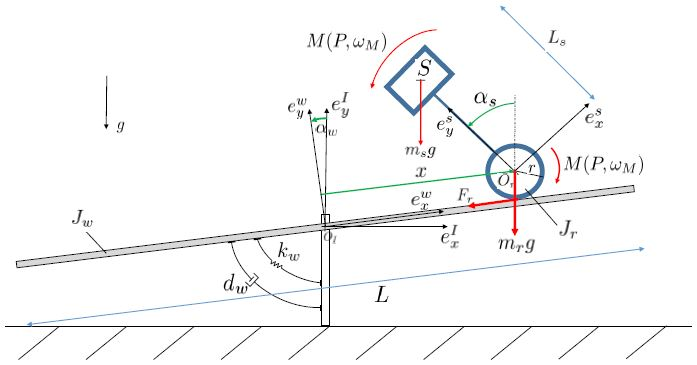
\includegraphics[width=\linewidth]{Bilder/SystematischerAufbau.jpg}}
	\caption{\textit{Systematischer Aufbau}}
\end{figure}


	\subsection{Wippe}
	Die Wippe hat eine rechteckige Auflage und ist 1.2m lang und 0.6m breit, auf 			welcher sich der Roboter vor- und zurückbewegen kann.
	Da die Bewegungsrichtung des Roboters nur einseitig erfolgt, ergibt sich daraus 		eine Beschränkung der Strecke von [-0.6, 0.6].
	Die Drehung der Wippe ist auf $\alpha^{}_{\omega}$ = [-$\frac{\pi}{6}$, $\frac{\pi}{6}$] beschränkt.
	Die Mitte der Wippe ist dabei die dunkelste Stelle des Farbverlaufs (vgl. Abb. \ref{fig:Helligkeit}).
	
	
	\begin{figure}[h]	
	\centerline{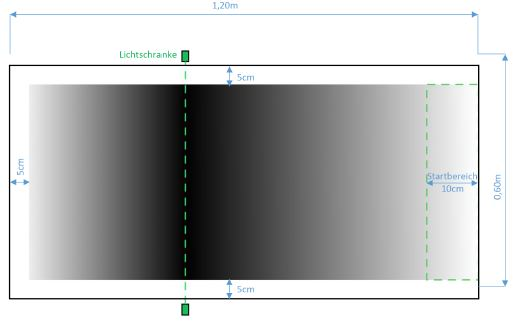
\includegraphics[width=\linewidth]{Bilder/Farbverlauf.jpg}}
	\caption{Helligkeitsverlauf}
	\label{fig:Helligkeit}
	\end{figure}
	
	\subsection{Segway}
	Die Raddrehung des Segways wird ohne Schlupf und ohne Reibung angenommen und der 		Schwerpunkt der Gesamtmasse ist im Punkt S konzentriert. 
	In der Regelungsaufgabe ist die absolute Drehung des Segways zur Vertikalen auf 		$\alpha^{}_{s}$ = [-$\frac{7\pi}{6}$, $\frac{7\pi}{6}$] beschränkt. %? 

	\subsection{Zustandsraum}
	%Erwähne die Komponenten der generalisierten Koordinaten
	%sechs Zustände
	Mit Hilfe der Lagrange-Gleichungen zweiter Art lässt sich das System mechanisch 		im Zeitbereich beschreiben und daraus ein Zustandsraum herleiten.
	Dabei hat der Zustandsvektor folgende Form:
	z = [$\alpha^{}_{\omega}$ $\dot{\alpha^{}_{\omega}}$ x \.{x} $\alpha^{}_{s}$ $\dot{\alpha^{}_{s}}$]%^{T} \\
	$\alpha^{}_{\omega}$: Winkel\\
	$\dot{\alpha^{}_{\omega}}$: Drehgeschwindigkeit der Wippe\\
	x:  Position der Radachse\\
	\.{x}:  Drehgeschwindigkeit des Rades\\
	$\alpha^{}_{s}$: absoluter Drehwinkel des Segways zur Vertikalen\\
	$\dot{\alpha^{}_{s}}$: absolute Drehgeschwindigkeit des Segways\\
	
		\subsubsection{Messgrößen}
		Mittels des Lichtsensors wird die Position der Radachse \textit{x} über den 		Farbverlauf der Wippe gemessen. Der eingebaute Gyroskop misst die absolute Drehgeschwindigkeit $\dot{\alpha^{}_{s}}$ des Segways.
		
		\subsubsection{Stellgröße}
		Die uns zur Verfügung stehende Stellgröße entspricht der elektrischen Motorleistung des Segways. Diese ist auf 3.56 Watt (vgl. Tabelle) beschränkt.
		Hier wurde zwischen absoluter und relativer Leistung unterschieden. Mit Hilfe einer gegebenen Motorkennlinie für verschiedene Leistungsstufen ließen sich die Stellgrößenbeschränkungen aus den folgenden Zusammenhang ermitteln.
		%umwandlung rel. und abs. 

	
\section{Lösungsansatz}
%Our design procedure was based on the idea that accelerating a vehicle results in shorter lap times than braking a vehicle. For presentational conciseness, we have listed some important parameters in Table 1.
%Modellierung => Linearisierung

\begin{figure*}[h]	
\centerline{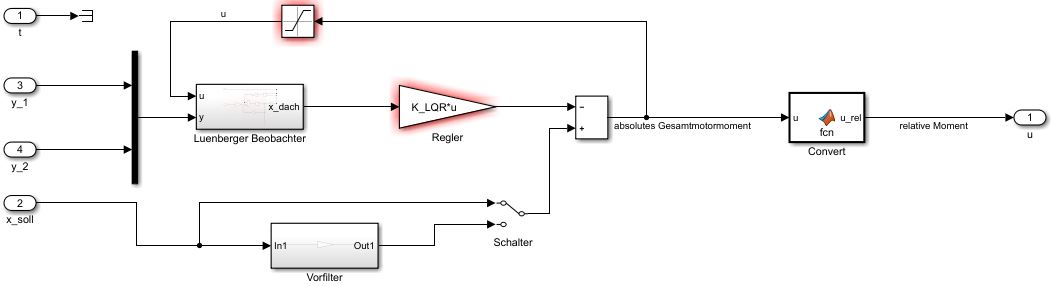
\includegraphics[width=\linewidth]{Bilder/Regler.jpg}}
	\label{fig:Regleraufbau}
	\caption{Regleraufbau im Simulinkmodell}
\end{figure*}


	\subsection{Linearisierung}
	%Anfangsbedinungen bzw. Ruhelagen alpha_s = 0 vgl. alpha_s = 0.5
	Die uns vorliegende Modellierung des Regelsystems ist nichtlinear, daher erlaubte dies uns keine einfache Implementierung einer Regelung nach den uns bekannten Methoden der Vorlesung ``Einführung in die Regelungstechnik''. 
	Eine Linearisierung des Systems um den stationären Arbeitspunkt ist daher nötig. Gegeben waren linearisierte Systemmatrizen, damit Folgefehler vermieden werden konnten. 
	
	\subsection{Stabilität}
	Wir haben das linearisierte System mittels MATLAB auf Stabilität überprüft. Da alle Eigenwerte negativ waren, ist asymptotische Stabilität garantiert.
	%evtl Eigenwerte
	
	\subsection{Zustandsregler}
	%LQR-Regler
	Da das linearistierte System steuerbar ist, sind die Pole der Strecke mittels eines Regler 			beliebig vorgebbar. Um die optimalen Sollpole zu finden, wurde ein LQR-Regler gewählt, 				welcher mittels der Gewichtungsmatrizen \textit{Q} und \textit{R} eingestellt wurde.
	Durch iteratives Vorgehen haben wir für Q eine Einheitsmatrix gewählt, was einer   					gleichstarken Gewichtung der Zustände entspricht. R wurde auf 1 gesetzt.
	


	%Regler mit nichtlinearen System zusammengeschaltet

	\subsection{Beobachter}
		Da am eigentlichen System nicht alle Zustände messbar sind, die für die Zustandsregelung 			mit dem LQR-Regler gebraucht werden, ist die Zuschaltung eines Beobachters nötig.
	Um diesen zu realisieren muss die Beobachtbarkeit des linearen Systems gewährleistet sein.
	Dies hat sich durch einer Analyse bestätigt.
	Hierzu haben wir die Struktur eines Luenberger-Beobachters eingesetzt und parallel zum            	Regelstreckenmodell geschaltet (vgl. Abb. \ref{fig:Regleraufbau}). Für die Wahl der Beobachterpole ist zu beachten, dass sich diese links der Pole des Zustandsreglers befinden, sodass die rekonstruierten Zustände den realen besser folgen. Um das verursachte Rauschen des Beobachters möglichst gering zu halten, dürfen die Pole wiederum nicht zu weit links gesetzt werden (vgl. Abb. \ref{fig:Rauschen1} und \ref{fig:Rauschen2}). Aufgrund dessen haben wir uns entschieden die Beobachterpole lediglich nur drei Einheiten weiter links der des Zustandsreglers zu setzen, da diese bereits sehr klein waren. 
	
	
	\begin{figure}[H]	
\centerline{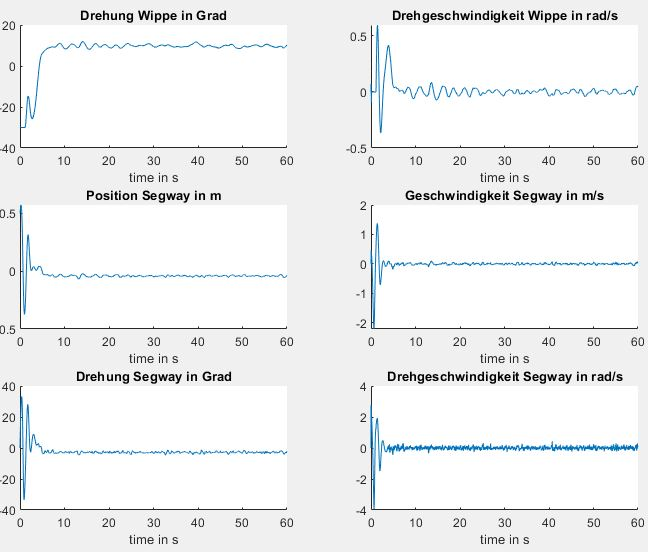
\includegraphics[width=\linewidth]{Bilder/Regler1.jpg}}
	\caption{Pole um drei Einheiten nach links}	\label{fig:Rauschen1}
\end{figure}

\begin{figure}[H]	
\centerline{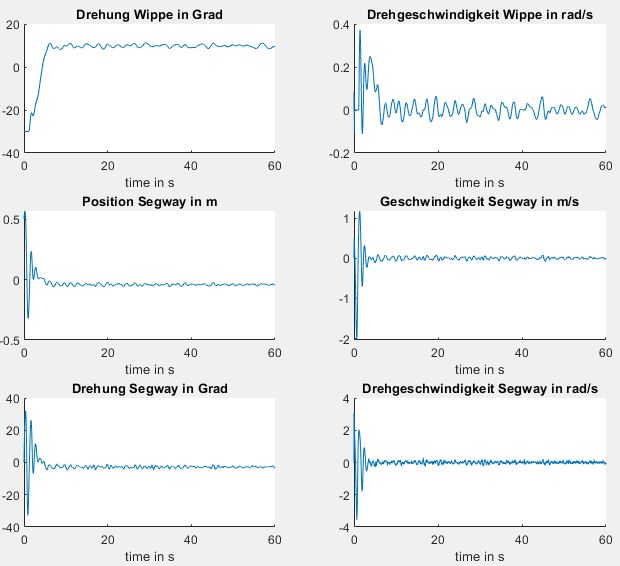
\includegraphics[width=\linewidth]{Bilder/Regler1mal2.jpg}}
	\caption{Pole um das doppelte nach links}	\label{fig:Rauschen2}
\end{figure}



	%Zustandsrückführung mit Beobachter verbinden 

	\subsection{Vorfilter}
	%Regelaweichung => Vorfilter
	%Wettbewerbsaufgabe für andere Ref größen
	%Plots mit und ohne Vorfilter bei 0.2 Refgröße
	%Ruhelage ist kein Vorfilter nötig
	%Abweichung mit Vorfilter bleibende RA 0.03 ohne Vorfilter bleibende RA 0.25
	%Ist aufgrund der rekonstruierten Zustände vllt noch zu verantworten
	Aus der Wettbewerbsaufgabe geht hervor, dass das Segway die Wippe nicht nur in der Mitte, sondern auch für andere Referenzpositionen $x^{}_{ref}$ = 0 stabilisieren soll. Wird die Referenzposition $x^{}_{ref}$ ungleich 0 gewählt, kommt es zu einer bleibenden Regelabweichung. Dieses Problem wird mit einem Vorfilter gelöst (vgl. Abb. \ref{fig:MitVorfilter} und \ref{fig:OhneVorfilter}). Wie zu erkennen ist, 
	ungeachtet des implementierten Vorfilters, ist noch eine bleibende Regelabweichung von ca. 0.03 Einheiten festzustellen. Dies scheint sich auf dem Beobachter zurückzuführen, weil dieser die Zustände nicht exakt rekonstruieren kann.  

\begin{figure}[h]	
\centerline{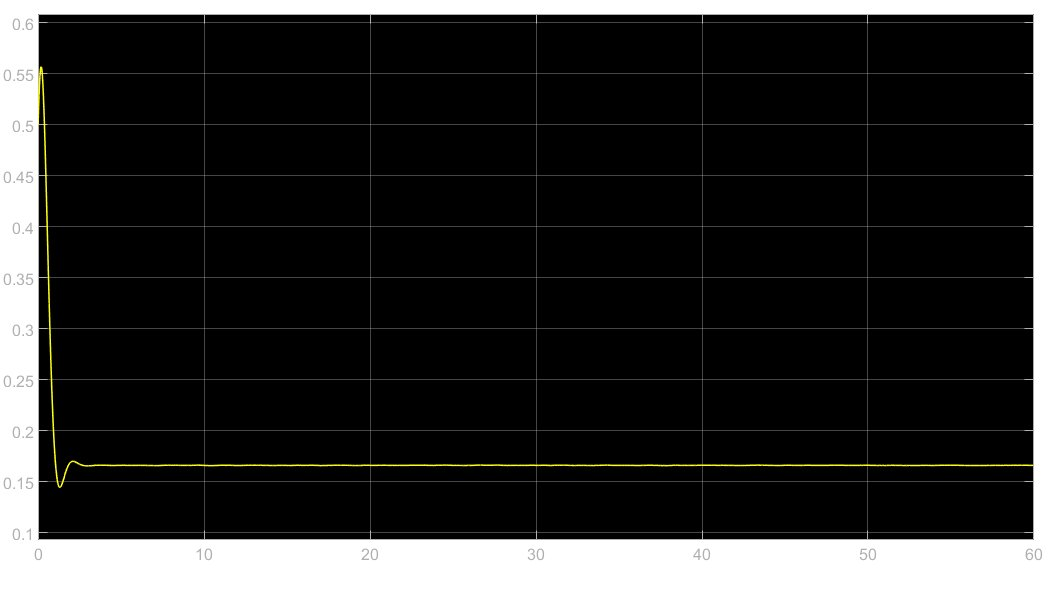
\includegraphics[width=\linewidth]{Bilder/Plots/MitVorfilter.jpg}}
	\caption{Mit Vorfilter}
	\label{fig:MitVorfilter}
\end{figure}

\begin{figure}[h]	
\centerline{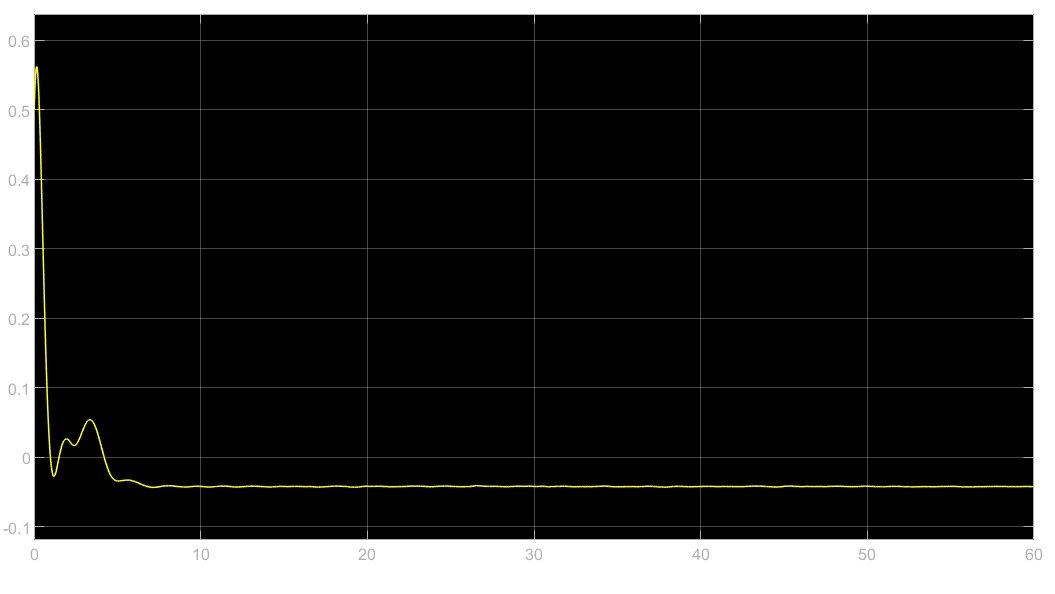
\includegraphics[width=\linewidth]{Bilder/Plots/OhneVorfilter.jpg}}	
	\caption{Ohne Vorfilter}
	\label{fig:OhneVorfilter}
\end{figure}




\section{Fazit}

%was erreicht?
%sollposition
%Anfangsbedingung 0.5 wegen rand besser als 0
Unsere Ziele: 1. Stabilisierung des Segways um dessen instabilen Ruhelagen (damit des Swegway nicht umkippt) 2. Regelung der Position des Segways auf der Wippe (mit der Begrenzung der Dimension der Wippe) wurden durch die folgenden Punkte erreicht:

\begin{itemize}
\item Mathematische Modellbeschreibung (Herleitung der Bewegungsgleichungen)  
\item Festlegung von nominellen Parameterwerten und Systemgrößen mit ihren Begrenzungen  
\item Linearisierung des nicht-linearen mathematischen Modells um die Ruhelage
\item Reglerentwurf
\item Beobachterentwurf
\item Implementierung von einem Vorfilter
\end{itemize}

Sollpositionen werden fast immer erreicht, obwohl diese variiert werden können. Diese kann man im Simulink Modell beliebig eintragen.

Zudem stellte sich heraus, dass durch die Wahl der Anfangsbedingung $\alpha^{}_{s}$ auf 0.5 Grad unserer Regler eine bessere Performance zeigt als mit 0 Grad.  

\begin{figure}[h]	
\centerline{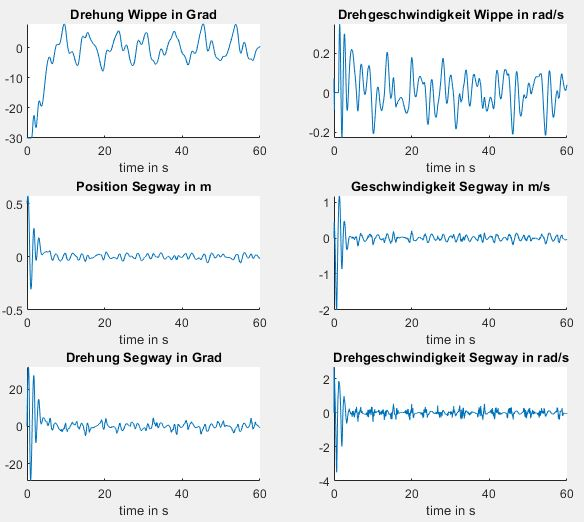
\includegraphics[width=\linewidth]{Bilder/Alf0undRef0.jpg}}
	\label{fig:Alf0undRef0}
	\caption{\textit{$\alpha^{}_{s}$ = 0}}
\end{figure}

\begin{figure}[h]	
\centerline{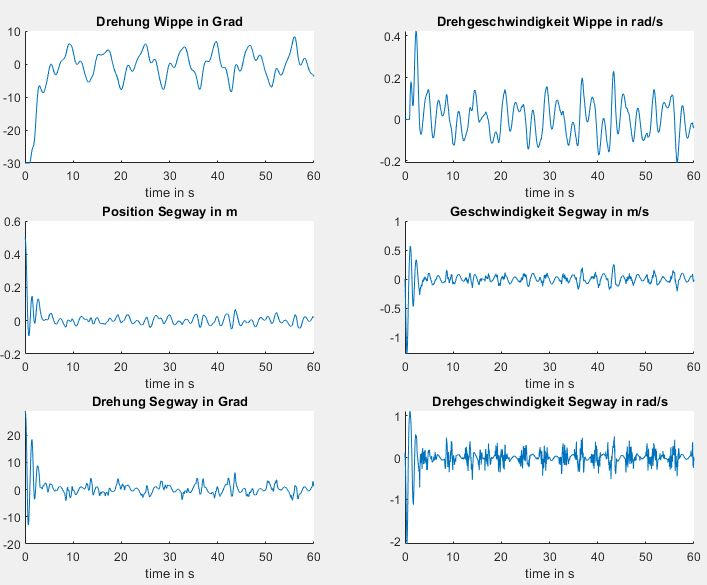
\includegraphics[width=\linewidth]{Bilder/Alf05undRef0.jpg}}
	\label{fig:Alf05undRef0}
	\caption{\textit{$\alpha^{}_{s}$ = 0.5}}
\end{figure}



\bibliography{Literatur}


%\begin{thebibliography}{3}
%
%\bibitem[(Knuth2005)]{Knuth2005}
%Knuth,~D.~E. (2005).
%\newblock The Art of Computer Programming.
%\newblock Pearson Education.
%
%\end{thebibliography}

%\appendix
\end{document}